\section{Extracellular conductivity}
\label{sec:Sigma}
\index{Extracellular conductivity}
\ghnote{GH: Planen var at dette skulle bli Torbjorns kapittel, men jeg laget en skisse.
Fint om Torbjorn sjekker alt jeg har foretatt meg, samt fyller ut med egne greier. Jeg sakset en del greier fra VC-kapittelet inn hit, blant annet delkapitlene om anisotropt og inhomogent medium. Pros: Naa utvider vi VC-teori i traad m/ at vi diskuterer (or relaxer) antakelser rundt sigma, jmf. tidligere versjon der vi utvidet VC teorien foerst, og deretter diskuterte og relaxet antakelsene. Cons: Naa blir det VC teori ogsaa i Sigma-kapittelet.}

A key parameter, or sometimes, variable, in volume conductor (VC) theory is the extracellular conductivity, $\sigma$. In most applications of VC theory, $\sigma$ is assumed to be a constant. Its value is normally taken from some experimental measurement, and typical recorded values are between 0.2 and 0.3 S/m (Fig. \label{Sigma:fig:freq_dep}). \ghnote{GH: Paastanden stemmer m/ figuren, men jeg har ikke oversikt over andre estimater som finnes der ute.} 

Throughout the previous section, we assumed that  $\sigma$  was homogeneous, anisotropic and frequency independent. In this chapter we shall discuss these assumptions. In addition, we discuss some experimental and theoretical estimates of  $\sigma$. 


%%%%%%%%%%%%%%%%%%%%%%%%%%%%%%%%
\subsection{\blue{Anisotropic extracellular medium}}
\label{sec:Sigma:Anisotropic}
%%%%%%%%%%%%%%%%%%%%%%%%%%%%%%%%
In Chapter \ref{sec:VC}, we assumed that the extracellular conductivity $\sigma$ was isotropic, i.e., the same in all spatial directions. It is relatively straightforward to expand the VC theory to the case of an anistotropic $\sigma$. If we use the point source approximation (eq. \ref{VC:eq:pointsources}), and denote the conductivity in the different spatial directions $\sigma_x$, $\sigma_y$ and $\sigma_z$, the extracellular potential surrounding a set of point current sources $I_k$ is given by \citep{nicholson1975, Pettersen2012}:

\begin{equation}
\phi(x,y,z) = \sum_k \frac{I_k}{4\pi(\sigma_y\sigma_z (x-x_k)^2 + \sigma_x\sigma_z (y-y_k)^2 + \sigma_x\sigma_y (z-z_k)^2)}.
\label{Sigma:eq:Panisos}
\end{equation}
If we use the CSD-description of the sources (eq. \label{VC:eq:csds}, the corresponding expression is:

\begin{equation}
\phi(x,y,z) = \iiint_V \frac{C(x,y,z)}{4\pi(\sigma_y\sigma_z (x-x_k)^2 + \sigma_x\sigma_z (y-y_k)^2 + \sigma_x\sigma_y (z-z_k)^2)} \, dV, 
\label{Sigma:eq:Canisos}
\end{equation}

In general, the brain does not have an isotropic $\sigma$. For example, in cortex it has been found that the conductivity is about 50\% higher in the depth direction, i.e., for currents running in parallel to the axis of pyramidal cell dendrites \citep{Goto2010}. However, the overall effect of the anisotropy on extracellular potentials often appears to be quite weak \citep{Ness2015}, and the approximation that $\sigma$ is isotropic often gives good predictions of the potential.


%%%%%%%%%%%%%%%%%%%%%%%%%%%%%%%%
\subsection{\red{TVN: Nonhomogeneous extracellular medium}}
\label{sec:Sigma:nonhomo}
In Chapter \ref{sec:VC}, we assumed that the extracellular conductivity $\sigma$ was homogeneous, i.e., the same everywhere. Clearly, this assumption does not hold on the micrometer scale, where neural tissue is highly non-homogeneous \citep{Nicholson1998}. However, microscale inhomogeneities tend to average out on a larger spatial scale (cf. the continuous medium approximation), and a homogeneous conductivity appears to be a reasonable approximation, at least within a given brain region such as cortex \citep{Logothetis2007}. 

The situation is different when signals are recorded very far from their sources. It is then likely that they on their journey have experienced a $\sigma$ that varied on a macroscopic scale. For example, the signals recorded in the EEG have traveled through brain tissue, bone and skin, which are three different media with different conductivities. When $\sigma$ is non-homogeneos, there is no general analytical formula available (like eqs. \ref{VC:eq:csds} or \ref{VC:eq:anisos}) that link the extracellular potentials to the underlying current sources. However, analytical solutions can still be obtained for some simple and idealized non-homogeneous cases. 

\ghnote{Enter TVN:}
\begin{itemize}
\item Method of Images \citep{Ness2015}
\item FEM \citep{Ness2015}, ...
\end{itemize}

For more general cases, one can in principle always solve eq. \ref{VC:eq:CSD2} for arbitrarily complex geometries with varying conductivities using numerical methods, like the Finite Element Method (FEM) \citep{Logg2012}. For examples of neuroscience applications using this approach, see \citep{Moffitt2005, Frey2009, Joucla2012, Haufe2015, Ness2015, Buccino2019b, Obien2019}. 

%%%%%%%%%%%%%%%%%%%%%%%%%%%%%%%%

\subsection{\orange{TVN: Frequency dependence of the conductivity} }
\label{sec:Sigma:f-independent}
\ghnote{GH: Skrev skisse til dette. Puttet figuren m/ sigma-maalinger inn her, da disse ser ut til aa primaert diskuteres opp mot eventuell frekvensavhengighet. Mulig vi burde ha med "eksperimentelle maalinger i kapittel-tittelen?}

Regardless of whether a medium is isotropic and homogeneous or not, its response to an imposed alternating current can depend on the frequency of the current. Then, the conductivity contains a resistive part, which is real and frequency independent, and an imaginary part that account for capacitive and inductive effects that are frequency dependent. 

In Section \ref{sec:VC:onlyohmic}) we argued that the extracellular displacement current is negligible, which means that the extracellular medium in itself does not exhibit any capacitive effects. This alone does not rule out the possibility that the effective conductivity of the tissue medium includes capacitive effects, as an extracellular current traveling through it could interact with nearby capacitive neural membranes. 

However, for the relevant frequencies in extracellular recordings (Fig. \ref{Sigma:fig:freq_dep}), the capacitive and inductive effects appear to be negligible compared to the resistive effects \citep{Logothetis2007, Miceli2017, Ranta2017}. In most applications of VC theory, one therefore applies the assumption that the medium is Ohmic or resistive, meaning that the imaginary and frequency dependent part of the conductivity is zero. We note, however, that it is possible to expand the formalism to include a frequency dependent conductivity \citep{Bedard2004, Tracey2011, Miceli2017}. 

\begin{figure}[!ht]
\begin{center}
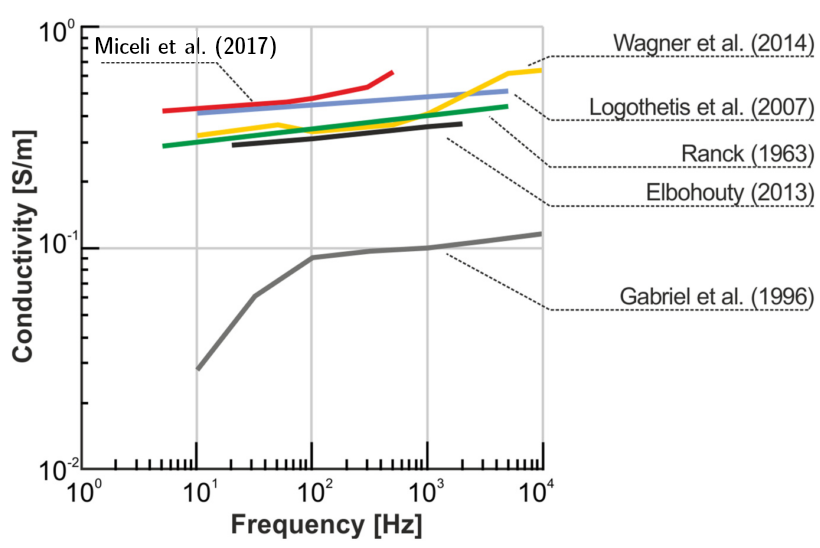
\includegraphics[width=0.6\textwidth]{Figures/Sigma/frequency_dependence.png}
\end{center}
\caption{\textbf{Literature review of reported conductivities in various species and experimental setups.} 
Most studies seem to indicate a very weak frequency dependence of the extracellular conductivity\index{conductivity}, which would have a negligible effect on measured extracellular potentials \citep{Miceli2017}. The very low and strongly frequency dependent values measured by \citep{Gabriel1996} represents an outlier, and although it has received substantial attention, it has to the best of our knowledge not been reproduced by any other study. For details about the data, see \citep{Miceli2017}, and references therein \citep{Ranck1963, Gabriel1996, Logothetis2007, Elbohouty2013, Wagner2014}.
}
\label{Sigma:fig:freq_dep}
\end{figure}

\tvnnote{Utledning tilsvarende Appendix B i Nunez?}
\ghnote{Vet ikke helt.... Kanskje.... }


\begin{figure}[!ht]
\begin{center}
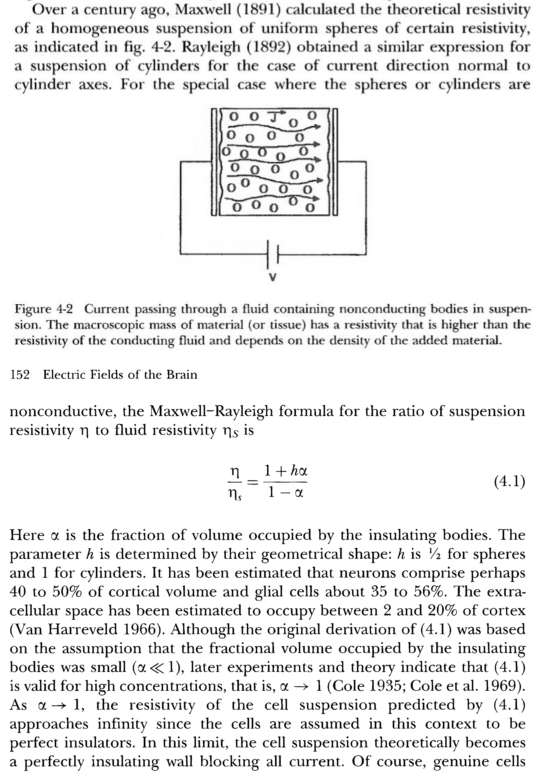
\includegraphics[width=0.6\textwidth]{Figures/Sigma/resistivity_maxwell.png}
\end{center}
\caption{\textbf{From Nunez} \tvnnote{Ta med noe slikt?}}
\label{Sigma:fig:maxwell_resistivity}
\end{figure}

\subsection{\orange{TVN: Theoretical explorations....} }
\ghnote{I den opprinnelige planen sto det at vi skulle skrive om dette, med referenser til Meffin2012, Tahayori2012, Meffin2014, Tahayori2014. Jeg vet ikke helt hva dette gaar i, men det gjoer sikkert Torbjorn og/eller Gaute?}

\subsection{\orange{GH: Theoretical estimate of the conductivity based on ion concentrations} }
\label{sec:Sigma:concentrationbased}
Extracellular current are mediated by the ions dissolved in the extracellular solution, and the conductivity of the extracellular medium if thus a function of thus depends on the ion concentrations, i.e., on the availability of free charge carriers \citep{Grodzinsky2011}: 

\begin{equation}
\sigma = \frac{F^2}{RT}\sum_{k} D_k z_{k}^2 c_{k}.
\label{Sigma:eq:sigma1}
\end{equation}
Here $z_{k}$, $D_k$ and $c_{k}$ denote the valency, diffusion coefficient and concentration, respectively, of ion species $k$, while $F = 96485.3$ C/mol is the Faraday constant, $R = 8.314$ JK$^{-1}$mol$^{-1}$ is the gas constant, and $T$ the temperature. 

Eq. \ref{Sigma:eq:sigma1} allows us to compare the measured $\sigma$ with the $\sigma$ predicted from the typical ion concentrations in the extracellular space of the brain, such as those listed previously in Table \ref{table:ion-concentrations}. For this, we also need the diffusion constants of these species. In a dilute solution, such as the extracellular fluid, these are as given in Table \ref{Sigma:tab:diffconsts}.

\begin{table}[h!]
\begin{center}
\caption{Diffusion constants. Values taken from from \citep{Bowen2002, Lyshevski2007}}
\label{Sigma:tab:diffconsts}
    \begin{tabular}{l|l}
    \hline
    $D_{Na}$ & $1.33\times 10^{-9}$ m$^2$/s\\ \hline
    $D_K$ & $1.96  \times 10^{-9}$ m$^2$/s \\ \hline
    $D_{Cl}$ & $2.03 \times 10^{-9}$ m$^2$/s \\ \hline
    $D_{Ca}$ & $0.71\times 10^{-9}$ m$^2$/s \\ \hline
    $D_{Mg}$ & $0.72\times 10^{-9}$ m$^2$/s \\ \hline    
    \end{tabular}
\end{center}
\end{table}

If we insert the values from Tables \ref{table:ion-concentrations} and \ref{Sigma:tab:diffconsts} into equation \ref{Sigma:eq:sigma1}, and assume a body temperature of $T = 310$ K, we get a conductivity $\sigma = 1.56$ S/m. This is a factor 5-8 times higher than the values (0.2-0.3 S/m) which are typically measured for the tissue conductivity. The discrepancy is mainly due to the fact that currents through brain tissue do not move through a free ion solution, but are (i) confined to stay in the small fraction of the tissue volume that is extracellular. In addition, (ii) the currents will face obstacles (neural and glial membranes) along their path, forcing them take detours. This is commonly incorporated into the theory by introducing reduced, effective diffusion coefficients: 

\begin{equation}
\tilde{D_k} = \alpha \frac{D_k}{\lambda^2}, 
\label{Sigma:eq:diffconst}
\end{equation}
where the parameter $\alpha$ denotes the extracellular volume fraction, while $\lambda$ is called the tortuosity of the medium, and accounts for the obstacles to free diffusion \citep{Nicholson1998}. Typical values for $\alpha$ and $\lambda$ in brain tissue are 0.2 and 1.6, respectively \citep{Nicholson1981, Nicholson1998}. If we insert the effective diffusion constants into eq. \ref{Sigma:eq:sigma1} it reduces $\sigma$ to $0.122$ S/m. This is somewhat lower than the values that are typically measured for $\sigma$. The main explanation is probably that we have underestimated $\sigma$ by only including the main charge carriers from Table \ref{table:ion-concentrations} in our calculation. The extracellular solution contains many ions (such as e.g., H$^+$ and HCO$_3$$^-$) besides these, which also will contribute to the conductivity. 

\ghnote{Forklaringen i siste setning er sikkert bra, men det finnes muligens andre? Deler av stroemmen gaar gjennom nevroner? }

As we shall see in Chapter \ref{sec:Eldiff}, the definition of $\sigma$ given by eq. \ref{Sigma:eq:sigma1} follows naturally if we use the Nernst-Planck equation for electrodiffusive ion concentration dynamics to compute extracellular currents. 
